\chapter{Analýza}

Na začátku této kapitoly je uvedena klíčová definice požadavků na funkcionalitu aplikace. V kontextu požadavků zmapujeme existující webové stránky s~recepty a~provedeme diskuzi nad jejich funkcemi, možnými vylepšeními a~rozšířeními. Následně rozebereme různé alternativy dostupných datových sad a~srovnáme jejich výhody i~nevýhody vzhledem k~požadavkům aplikace.

\section{Požadavky aplikace}

Požadavky na aplikaci lze rozdělit do skupiny funkčních a~nefunkčních. Funk\-ční požadavky popisují konkrétní funkcionalitu systému, zabývají se vstupem od uživatele a~prezentací výstupu. Díky tomu je lze poměrně snadno definovat a~testovat jejich naplnění v hotové aplikaci. Nefunkční požadavky se naopak na konkrétní vstup nevážou a~místo toho popisují vlastnosti a~omezení, které by měl systém splňovat. Zjednodušeně lze říci, že funkční požadavky popisují, co má systém dělat, zatímco nefunkční požadavky specifikují, jaký má systém být \citep{app-requirements}.

\subsection{Funkční požadavky}

Následuje výčet funkcionalit, které by aplikace svým uživatelům měla nabídnout. Uživatelé mohou mít různé role od běžného návštěvníka stránky po administrátora nebo vývojáře integrujícího data do jiného systému.

\subsubsection{Běžný uživatel}

\begin{enumerate}
    \item Aplikace poskytuje uživatelské rozhraní pro vyhledávání receptů na základě ingrediencí, klíčových slov, času přípravy, hodnocení a~nutričních hodnot.
    \item Aplikace umožňuje kombinovat libovolné množství vyhledávacích filtrů.
    \item Aplikace podporuje zadávání vlastních i~předdefinovaných ingrediencí prostřednictvím našeptávače.
    \item Aplikace podporuje fasetové vyhledávání, tedy u~nabízených možností zobrazuje počet receptů, které se po zvolení daného filtru zobrazí.
    \item Aplikace poskytuje možnost smazání všech vyhledávacích filtrů jedním kliknutím, ale také mazání po jednom filtru.
    \item Aplikace zobrazuje uživateli všechny nalezené výsledky bez omezení na maximální počet výsledků.
    \item Aplikace při otevření vyhledávací obrazovky bez zadaných filtrů zobrazuje všechny recepty, které má v~databázi.
    \item Aplikace umožňuje zobrazení detailu receptu bez přesměrování na zdrojovou stránku.
    \item Aplikace zobrazuje pouze recepty s~titulní fotografií.
    \item Aplikace na vyhledávací stránce pro každý nalezený recept zobrazuje jeho název, popis, obrázek, čas přípravy, hodnocení a~počet recenzí.
    \item Aplikace nabízí náhledy všech ingrediencí u~vyhledaných receptů a~zvýrazňuje aktuálně vyhledávané ingredience.
    \item Aplikace umožňuje listování nalezenými výsledky prostřednictvím systému stránkování, nikoli nekonečným posouváním stránky.
    \item Aplikace plně podporuje navigaci v~rámci historie prohlížeče včetně přidávání a~odebírání filtrů i~listování více stranami výsledků.
    \item Aplikace na detailní stránce každého receptu zobrazuje název, hodnocení, počet recenzí, popis, čas přípravy, fotografii, ingredience, postup přípravy a~nutriční hodnoty.
    \item Aplikace zvýrazňuje ingredience na detailní stránce receptu, ke kterým má dodatečné informace.
    \item Aplikace přesměrovává na obrazovku s~detailem ingredience po kliknutí na zvýrazněnou ingredienci.
    \item Aplikace zobrazuje na detailní stránce ingredience následující informace nebo jejich podmnožinu: název, popis, obrázek, nutriční hodnoty, náhrady, kategorie a~níže recepty obsahující tuto ingredienci, které lze otevřít stejně jako z~vyhledávací obrazovky.
    \item Aplikace má nezávisle na otevřené stránce viditelný ovládací panel s~možností navigace na vyhledávací obrazovku.
\end{enumerate}

\subsubsection{Externí systém}

\begin{enumerate}
    \item Aplikace poskytuje REST API endpointy pro získání dat k~receptům a~ingrediencím.
    \item Aplikace zpřístupňuje JSON-LD reprezentaci dat v~hlavičkách dokumentů s~recepty a~ingrediencemi.
    \item Aplikace podporuje navigaci a~vyhledávání receptů přes url adresy s~query parametry.
\end{enumerate}

\subsection{Nefunkční požadavky}

Požadavky z~této kategorie lze dále dělit podle jejich zaměření. Některé se věnují výkonu aplikace, jiné spolehlivosti, přenositelnosti, bezpečnosti, využitým technologiím, vývojovému prostředí nebo platformě, testovatelnosti či rozšiřitelnosti. Oblastí je zde skutečně mnoho, uvedeme proto pouze výčet konkrétních požadavků na naši aplikaci.

\begin{enumerate}
    \item Backend aplikace je postaven na frameworku Express.js pro Node.js prostředí.
    \item Frontend aplikace je implementován pomocí knihovny React.
    \item Backend i~frontend aplikace jsou psány staticky typovaným jazykem\newline TypeScript.
    \item Aplikace využívá dokumentovou databázi Apache CouchDB pro uložení dat o~receptech a~ingrediencích.
    \item Aplikace využívá systém Apache Solr pro implementaci vyhledávání receptů.
    \item Aplikace využívá program Silk Workbench pro objevování linků mezi dvěma entitami.
    \item Aplikace je implementovaná jako single-page aplikace s~podporou routingu mezi více obrazovkami.
    \item Aplikace integruje data z~aspoň 2 různých veřejných znalostních grafů.
    \item Aplikace pro komunikaci mezi klientem a~serverem používá REST API v~kombinaci s~asynchronními požadavky. 
    \item Uživatelské rozhraní aplikace je založeno na knihovně Material UI poskytující sadu univerzálních komponent pro React aplikace.
    \item Uživatelské rozhraní aplikace je responzivní pro desktopová i~mobilní zařízení.
    \item Databáze obsahuje v~prvotní fázi přes $50\,000$ receptů z~aspoň $2$ různých zdrojů.
    \item Aplikace je škálovatelná co do množství poskytovaných dat.
    \item Aplikace je škálovatelná z~pohledu nových lokalizací a~jejich distribuce.
    \item Aplikace je připravena pro implementaci nových rozšíření bez nutnosti výrazné změny stávajícího kódu.
    \item Vyhledávání receptů je pro nového uživatele přímočaré a~filtrování zvládne nastavit v~řádu vteřin v~závislosti na počtu požadovaných filtrů.
    \item Zdrojový kód aplikace je open-source a verzovaný na platformě GitHub.
    \item Zdrojový kód aplikace je přehledný a~snadno rozšiřitelný dalšími vývojáři.
    \item Komponenty aplikace jsou znovupoužitelné v~rámci projektu i~mimo něj.
    \item Získání receptů pro jednu stránku výsledků trvá méně než $500\,\rm ms$ ($200\,\rm ms$ dotaz na server, $200\,\rm ms$ doručení odpovědi klientovi a~$100\,\rm ms$ rezerva).
    \item Rendering jedné stránky vyhledaných receptů trvá méně než $1\,000\,\rm ms$ od načtení dat do paměti.
    \item Nově extrahovaná data se uživatelům aplikace zobrazí nejpozději do druhého dne. 
    \item Aplikace je kompatibilní s~webovými prohlížeči Google Chrome, Mozilla Firefox a~Microsoft Edge.
\end{enumerate}

\subsection{Uživatelské příběhy}

Požadavky aplikace lze méně formálním způsobem popsat pomocí tzv. uživatelských příběhů, které vyjadřují přání a očekávání uživatele vůči aplikaci. Uživatel vyžaduje konkrétní funkcionalitu pro dosažení vybraného cíle. Uživatelské příběhy jsou důležitou součástí agilního vývoje, neboť kladou důraz na potřeby uživatele, které se v průběhu vývoje mohou vyvíjet a měnit. Obvykle příběhy zapisujeme v jednoduchém formátu: \uv{Jako (role) chci (funkce)[, abych (cíl)]} \citep{user-stories}. Následují příklady uživatelských příběhů v kontextu naší aplikace:

\begin{enumerate}
    \item Jako kuchař, který má vybraných několik hlavních ingrediencí, chci najít všechny recepty obsahující tyto suroviny.
    \item Jako milovník řecké a~italské kuchyně chci použít filtrování receptů z~těchto oblastí, abych nemusel procházet detaily receptů a~hledat jejich původ v~popisu.
    \item Jako uživatel, který rád šetří čas, chci znát všechny ingredience daného receptu ještě před otevřením jeho detailu, abych se vyhnul čtení receptů s~příliš mnoha dodatečnými ingrediencemi.
    \item Jako zaneprázdněný student chci snadno najít recepty, které lze připravit za méně než $30$ minut.
    \item Jako celiak chci hledat pouze recepty bez obsahu lepku.
    \item Jako vrcholový sportovec chci snadno najít recepty s~vysokým obsahem bílkovin.
    \item Jako nutriční poradce chci u~receptů vidět podrobný rozpis nutričních hodnot, abych daný recept mohl doporučit svým klientům dle jejich stravovacích potřeb.
    \item Jako hostitel očekávající návštěvu potřebuji znát počet porcí, které se základním množstvím surovin připravím, abych toto množství mohl přizpůsobit počtu hostů.
    \item Jako zvídavý uživatel se chci při čtení receptu dozvědět zajímavosti o~jeho ingrediencích.
    \item Jako uživatel s~vytříbeným vkusem chci hledat pouze recepty s~maximálním hodnocením a~s~co největším počtem kladných recenzí.
    \item Jako nerozhodný uživatel chci mít možnost rychlé změny vyhledávacích filtrů.
    \item Jako uživatel, který našel zajímavý recept před několika dny, chci využít historii prohlížeče a~najít recept dle názvu, abych nemusel vzpomínat na vyhledávací filtry, pomocí nichž jsem recept původně objevil.
    \item Jako kuchař spokojený s~připraveným pokrmem chci najít autora receptu a~vyhledat jeho další recepty.
    \item Jako uživatel s~preferencí vzhledu Material Design bych rád pracoval s~aplikací, která je na tomto stylu založená.
    \item Jako vývojář externí aplikace s~recepty bych rád jednoduše získal strukturovaná data receptů, abych každou informaci nemusel extrahovat přes jednotlivé CSS selektory.
    \item Jako webový vyhledávač potřebuji informace k receptům ve strukturovaném formátu pro Linked Data, ideálně popsané dle entity \texttt{Recipe} z ontologie Schema.org.
\end{enumerate}

\section{Dostupné datové sady}

V~této sekci je vyhrazen prostor pro analýzu různých veřejně dostupných datasetů z~domény receptů. Nejedná se ani zdaleka o~kompletní výčet, měly by ale být představeny nejznámější alternativy, které by mohly být vybrány jako podklad pro obsah aplikace. 

\subsection{Recipe1M+}

Jedním z~nejdůležitějších projektů v~této oblasti je \emph{Recipe1M+}, strukturovaný korpus obsahující přes $1$~milion receptů a $13$ milionů souvisejících obrázků jídla. Aktuálně se jedná o~největší veřejně dostupnou sadu receptů. Dataset je dostupný pouze přihlášeným uživatelům z~ověřené organizace a je povoleno jej využívat výhradně pro účely studia a výzkumu. Pro registraci lze využít univerzitní email. Z~celkového počtu $1$~milionu receptů obsahuje $50\,000$ receptů s~nutričními informacemi \citep{marin2019learning}. V~naší aplikaci preferujeme nutriční hodnoty zahrnout, pokud jsou dostupné na zdrojové stránce receptu. Měli bychom tedy k~dispozici $50\,000$ dokumentů s~touto informací. Ostatní data jsou určena přednostně pro strojové zpracování prostřednictvím trénování modelů.

Celková velikost datové sady se pohybuje v~řádu stovek gigabytů, samotné JSON dokumenty se strukturovanými recepty z~adresáře \texttt{layers} se ale vejdou do $2~GiB$, tudíž by byly vhodné pro potřeby této práce limitované omezenou výpočetní kapacitou. Lze odtud využít $1\,029\,720$ receptů obsahujících název, URL, ingredience a~postup přípravy. Odkazy na ilustrační fotografie jsou u~$402\,760$ z~těchto receptů. Pro příjemnější uživatelský zážitek se omezujeme pouze na recepty s~obrázky, takže jsme z~datasetu Recipe1M+ schopni použít přibližně $400\,000$ receptů, pokud akceptujeme absenci nutričních hodnot. Bylo by spíše obtížnější z~tohoto datasetu identifikovat názvy ingrediencí, neboť jsou suroviny uloženy včetně jejich množství a~jednotek měření v~rozmanitém formátu.

\subsection{Open Recipes}

Dalším významným aktérem na poli volně dostupných receptů je iniciativa \emph{Open Recipes}. Autoři Finkler, Shiflett a Birkebæk projekt představují jako otevřenou databázi záložek s~recepty. Pojem záložky je použit z~důvodu absence instrukcí k~přípravě receptu. Dataset má sloužit pouze k~vyhledání receptu a~pro detailní informace má být uživatel přesměrován na zdroj s~kompletním receptem \citep{open-recipes}. Tohoto přístupu úspěšně využívají některé z~vyhledávačů receptů, např. populární aplikace \emph{SuperCook}. Naše aplikace si ale klade za cíl zpracovat i~stránky s~detaily receptů, ze kterých lze dále pokračovat na detaily ingrediencí s~informacemi ze znalostních grafů. Projekt Open Recipes tedy pro náš scénář nebude vhodnou volbou.

\subsection{FoodKG}

Přímo v~oblasti znalostních grafů figuruje projekt \emph{FoodKG}, který je postaven nad sadou receptů z~již zmíněného datasetu Recipe1M+. Recepty doplňuje o~podrobnější data k~ingrediencím ze stránky The~Cook's~Thesaurus a~definuje vlastní ontologii. Model ontologie je navržen pro zodpovídání dotazů na recepty dle ingrediencí s~přihlédnutím k~individuálním potřebám uživatele, jako jsou alergie a~intolerance na určité složky potravin.

Vývojáři projektu FoodKG zpřístupňují skripty k~extrakci dat z~encyklopedie The~Cook's~Thesaurus a~k~vytvoření znalostního grafu. Neposkytují ale žádné nové recepty nad rámec datové sady Recipe1M+, naší horní hranicí by tedy bylo $50\,000$ receptů s~nutričními hodnotami (viz sekce \emph{Recipe1M+}). Ontologie publikovaná na webových stránkách projektu obsahuje $75$ entit ingrediencí, které kromě obecného popisu poskytují informace o~glykemickém indexu, obsahu lepku a~možných náhradách dané ingredience. Výhodou je připravený RDF formát, nad kterým se lze snadno dotazovat pomocí jazyka SPARQL. Autoři Chen~a~kol. uvádějí ukázky dotazů, vyberme například dotaz vracející recepty, které obsahují banán a~zároveň neobsahují vlašské ořechy \citep{food-kg}:

\begin{code}
@PREFIX food: <http://purl.org/heals/food/>
@PREFIX ingredient: <http://purl.org/heals/ingredient/>
SELECT DISTINCT ?recipe
WHERE {
    ?recipe food:hasIngredient ingredient:Banana .
    FILTER NOT EXISTS {
        ?recipe food:hasIngredient ingredient:Walnut .
    }
}
\end{code}
%$

\subsection{Food.com Recipes and Interactions}

Rozsáhlý dataset \emph{Food.com Recipes and Interactions} s~téměř $200\,000$ recepty extrahovanými z~webové stránky Food.com (původního GeniusKitchen) je publikován na portálu \emph{Kaggle}, který shromažďuje podklady pro strojové učení. Datová sada pokrývá $18$ let interakce uživatelů včetně hodnocení, počtu recenzí i~konkrétních reakcí \citep{shuyang_li_2019}. Kromě základních informací obsahuje také nutriční hodnoty receptů, datum publikování a~rovněž normalizovaná jména ingrediencí. Ta byla získána parsováním originálního textu surovin, kvůli čemuž nejsou vždy zcela spolehlivě přesná (např. ve jménech často zůstala jednotka měření z~původního textu). Unikátních ingrediencí je k~dispozici kolem $8\,000$, což by měl být dostačující základ pro hledání linků s~entitami otevřených znalostních grafů. Zároveň ve srovnání s~předchozími projekty nabízí nejbohatší informace k jednotlivým receptům.

Nevýhodou datasetu je jeho primární určení pro strojové zpracování. Byl vytvořen jako podklad pro generování personalizovaných receptů na základě dřívějších preferencí uživatele \citep{majumder-etal-2019-generating}. Syrová data nejsou zamýšlena pro přímou prezentaci, což se negativně odráží na jejich přesnosti a estetice. Slova jsou občas zařazena do špatných kategorií a~problematický je zejména plně \emph{lowercase} formát textu, ze kterého nejsme schopni zpětně zrekonstruovat originální text receptu. Dataset bychom tedy nemohli použít samostatně, ale pouze v~kombinaci s~vlastní extrakcí dat, která by respektovala velikost písma a~lépe se vypořádala s~parsováním jednotlivých kategorií.

Tento problém je poměrně snadno řešitelný díky struktuře stránky Food.com. Z~id receptu lze jednoduše složit URL ve formátu \texttt{www.food.com/recipe/id} a~navíc aplikace podporuje koncept propojených dat, tedy poskytuje recepty ve strukturovaném RDF formátu. Do HTML hlaviček všech dokumentů s~recepty vkládá JSON-LD serializaci dle ontologie \emph{Schema.org}. Z~připraveného datasetu bychom tedy mohli využít identifikátory receptů a~normalizované ingredience, pro každý recept extrahovat jeho JSON-LD a spojit informace dohromady. Zároveň bychom si ušetřili práci s~převáděním receptů do JSON-LD formátu a připravené soubory rovnou vložili do hlaviček dokumentů. Nevytvářeli bychom nové entity receptů, pouze bychom změnili prezentační vrstvu RDF dat. Identifikátory entit v podobě IRI by tedy zůstaly nezměněné.

\subsection{Generování vlastního datasetu}

Pokud se nespokojíme s~žádnou z~dostupných datových sad, případně potřebujeme data rozšířit a~posbírat je přímo ze zdroje, využijeme metodu zvanou \emph{web scraping}. V~rámci tohoto procesu musíme analyzovat cílovou stránku z~pohledu získávání a~prezentace dat. S~využitím vývojářským nástrojů ve webovém prohlížeči můžeme přes panel \texttt{Network} sledovat požadavky, které aplikace odesílá na svůj server a~v~mnoha případech se na toto interní API dokážeme napojit a~získat data ve strukturované podobě. Aplikace typicky pracují s~REST~API, GraphQL API nebo jejich kombinací a~standardně data poskytují ve formátu JSON. Pokud žádný požadavek typu fetch pro získávání potřebných dat neobjevíme, musíme informace extrahovat přímo z~HTML dokumentu prostřednictvím CSS selektorů. V~obou případech budeme aplikaci posílat GET požadavky, ať už na její backend pro strukturovaná data nebo na frontend pro HTML dokumenty k následnému parsování.

Problematická je kategorie aplikací, které data nezískávají s~využitím transparentních požadavků a~zároveň potřebují spouštět JavaScript kód pro vygenerování obsahu. Zde nestačí pouhé poslání GET požadavku přes HTTP, neboť odpověď neobsahuje žádná relevantní data uvnitř HTML. Pro zvládnutí tohoto typu stránek potřebujeme zapojit automatizaci webového prohlížeče. Nejznámějšími projekty, které se této automatizaci věnují, jsou Selenium\footnote{https://github.com/SeleniumHQ/selenium}, Puppeteer\footnote{https://github.com/puppeteer/puppeteer}, Playwright\footnote{https://github.com/microsoft/playwright} a~Cypress\footnote{https://github.com/cypress-io/cypress} pro automatizaci testování \citep{selenium-ecosystem}. Všechny ze zmíněných projektů jsou open-source.

Během posílání požadavků můžeme rovněž narazit na různé formy blokování, od limitu maximálního počtu požadavků z~jedné IP adresy přes povinné autorizační tokeny až po CAPTCHA testy řešitelné pouze s~využitím umělé inteligence. Některé aplikace navíc kontrolují tzv. otisk webového prohlížeče. Jedná se o~sadu informací k~zařízení uživatele, jmenovitě data o~konkrétním hardwaru, operačním systému a~webovém prohlížeči včetně konfigurace \citep{browser-fingerprints}. Také se při neopatrnosti může stát, že server aplikace zahltíme příliš velkým množstvím paralelních požadavků, čímž prodloužíme dobu odezvy nebo zpracování dalších požadavků dočasně zcela znemožníme.

Stejně jako v~jiných oblastech se hodí využít nástroj, který co nejvíce běžných problémů vyřeší za nás. Na poli open-source nástrojů pro extrakci dat si vedoucí pozici drží knihovna Scrapy\footnote{https://github.com/scrapy/scrapy} psaná v~jazyce Python, která nabízí celou řadu pokročilých funkcí proti blokování požadavků. Pro potřeby této práce by ale vzhledem k~rozsáhlejší osobní zkušenosti byla vhodnou volbou knihovna Apify\footnote{https://github.com/apify/apify-js} pro Node.js. V~arzenálu má zpracování HTTP požadavků s~následným parsováním HTML pomocí knihovny Cheerio\footnote{https://github.com/cheeriojs/cheerio}, ale také automatizaci webového prohlížeče s~využitím knihoven Puppeteer nebo Playwright, včetně generování otisků webového prohlížeče. Navíc zajišťuje rotaci IP adres, čímž snižuje množství zablokovaných požadavků. IP adresy lze v rámci placeného účtu získat přímo od firmy Apify, nebo na vstupu poskytnout seznam vlastních. Obecně preferujeme program nespouštět z~osobní IP adresy, neboť riskujeme, že nás stránka někdy i~natrvalo zablokuje, případně se naše IP adresa dostane na veřejný seznam adres doporučených k~blokování.

S~dostatkem času, výpočetních prostředků, IP adres pro rotování a~s~velikou kapacitou úložiště bychom byli schopni zpracovat většinu vybraných aplikací s~recepty. Pro každou stránku bychom napsali dedikovaný program a~postupně extrahovali data z~celé stránky. Recepty z~různých aplikací bychom uložili ve sjednoceném formátu a~výsledkem by byl kvalitní dataset s~maximálním množstvím dat, které lze od zdrojových stránek získat. Práce ovšem necílí na datovou sadu takovéto velikosti. Místo toho se zaměřuje na vytvoření infrastruktury nad podmnožinou receptů, kterou bude možné libovolně škálovat dle možností dalšího vývoje. V~případě vlastní extrakce dat bychom si tedy vybrali dva až tři zástupce aplikací, navrhli pro ně jednoduché řešení extrakce dat a~omezili počet sesbíraných výsledků na rozumnou hodnotu. Dle požadavků aplikace musíme zároveň splnit spodní limit více než $50\,000$ receptů. Vhodným kandidátem by jednoznačně byla zmíněná stránka Food.com, která v~době psaní této práce obsahuje přes $500\,000$ receptů a~pro cca $200\,000$ z~nich máme k dispozici unikátní identifikátory skrze dataset z~platformy Kaggle. Navíc dokumenty s~recepty obsahují JSON-LD reprezentaci v~hlavičce HTML. Pro každý recept se známým id by tedy stačilo vytvořit URL, poslat na něj GET požadavek a~z~HTML odpovědi extrahovat JSON-LD data. Podobně bychom mohli zpracovat recepty ze stránky Allrecipes, kde jsou v~detailech receptů rovněž publikována JSON-LD data. URL adresy receptů by mohl objevit přímo náš program během procházení stránky nebo bychom mohli využít sesbírané URL adresy z~datasetu Recipe1M+.

\subsection{DBpedia}

Znalostní graf DBpedia by mohl posloužit pro extrakci rozšiřujících informací k~ingrediencím nasbíraným z~jednotlivých receptů. Prvním krokem by byla identifikace názvů ingrediencí z~datasetu s~recepty. Ideální by bylo mít k~dispozici již extrahované ingredience, což není samozřejmostí, neboť recepty jsou často poskytovány bez strukturovaného textu surovin. Ten kromě názvu ingredience může obsahovat také její množství a jednotku měření. Není pak snadné spolehlivě určit, která část textu není součástí jména ingredience, zejména kvůli rozmanitým názvům jednotek měření. Nicméně i~jednotek je jen konečné množství a~s~dostatečným úsilím bychom je měli být schopni identifikovat. Pro každou novou lokalizaci bychom ale problém řešili znova. Strukturovaným ingrediencím s~odděleným názvem, množstvím a~jednotkou měření bohužel nenahrává standardizovaný formát receptu dle ontologie Schema.org\footnote{https://schema.org/Recipe}. Ten definuje typ vlastnosti \texttt{recipeIngredient} jako prostý text, tedy včetně množství a jednotky.

Jakmile by se nám podařilo získat určitou skupinu jmen surovin, vytvořili bychom jednoduché entity ingrediencí v~RDF formátu. Stačilo by každé surovině přiřadit unikátní IRI a~vlastnost typu \texttt{rdfs:label} odpovídající názvu dané ingredience. Z~těchto informací bychom sestavili RDF dataset a~nahráli jej do aplikace Silk Workbench. Následně bychom provedli konfiguraci DBpedia SPARQL endpointu a~nalezli shody s~hodnotami \texttt{rdfs:label} ve znalostním grafu DBpedia. Abychom se vyhnuli prohledávání celého grafu, potřebujeme nastavit omezení na povolený typ entit. Po zběžné analýze konkrétních instancí surovin na DBpedia můžeme využít např. následující jednoduché omezení, kde proměnná \texttt{?a} znázorňuje dle konvence Silk Workbench hledanou entitu:

\begin{code}
{ 
    {
        ?recipe <http://dbpedia.org/ontology/ingredient> ?a
    } UNION {
        ?a <http://dbpedia.org/ontology/ingredient> ?anotherIngredient
    } 
}
\end{code}
%$

Výše uvedený fragment dotazu cílí na všechny entity, které vystupují jako ingredience jiných entit a~zároveň z~opačného směru hledá všechny entity, které obsahují nějakou ingredienci. Z~dat na DBpedia totiž můžeme vypozorovat, že obsahuje nejen základní ingredience, ale také suroviny složené z~více přísad. Takové ingredience by bylo možné považovat za recept, nicméně i~ony mohou být dále použity v~rámci komplexnějšího postupu přípravy pokrmu. Dobrým příkladem složené ingredience je guacamole, které bývá často uváděno jako přísada (např. u~hamburgerů), ale samo je produktem z~avokáda, rajčat, cibule, česneku a~limetky.

Dále si potřebujeme zvolit podmnožinu informací, které chceme extrahovat a~uložit do vlastní databáze. Opět provedeme pozorování konkrétních instancí surovin a~identifikujeme názvy vlastností pro jméno, popis, obrázek, nutriční hodnoty, kategorie a~místo původu. Je třeba mít na paměti, že množství dat pro jednotlivé ingredience bude velmi proměnlivé a~i~jména vlastností nebo typ hodnot mohou být do určité míry odlišné. Do budoucna je zde prostor pro získání kvalitních dat pro rozdílné lokalizace aplikace, neboť ve znalostním grafu lze snadno filtrovat literály v požadovaném jazyce.

\subsection{Wikidata}

Práce se znalostním grafem Wikidata by probíhala velmi podobně jako u~výše popsaného projektu DBpedia. Pomocí Silk Workbench bychom vytvořili vazby mezi entitami ingrediencí a~následně extrahovali data k~nalezeným přísadám. Ve srovnání s~obsahem grafu DBpedia je zde většinou k~dispozici menší množství textu a~spíše je kladen důraz na odkazy do jiných zdrojů. Dle zběžného pozorování ale graf Wikidata často poskytuje relevantnější obrázky, kategorie a~místo původu. Také mnohdy uvádí obsažené složky (např. smetanu a~mléko u másla) a~u~vybraných ingrediencí zobrazuje barvu nebo dokonce Unicode znak.

Pokusíme se získat z~DBpedia i~Wikidata co nejvíce ze zmíněných informací a~sloučit je dohromady. Tím bychom měli vylepšit poměr ingrediencí, ke kterým najdeme větší množství zajímavých informací. Dotaz na stejnou vlastnost dané entity může totiž na DBpedia i~Wikidata dopadnout úplně jinak, přestože oba čerpají z~projektu Wikipedia.

\section{Úspěšné webové aplikace s recepty}

V~této sekci projdeme konkrétní příklady úspěšných webových aplikací z~domény vyhledávání receptů a~uvedeme, v~čem se od nich plánujeme odlišit a~které rozšiřující funkce naše aplikace nabídne. Stránek v~oblasti gastronomie a~přípravy pokrmů existuje velké množství, vybereme tedy podmnožinu těch nejznámějších na základě jejich pozice ve vyhledávaných výsledcích. Pro přibližnou analýzu návštěvnosti využijeme kombinaci dotazu \texttt{recipes by ingredients} ve vyhledávači Google, dále položíme stejný dotaz platformě Spyfu\footnote{https://www.spyfu.com/} a nakonec zkontrolujeme kategorii \texttt{Cooking and Recipes} na stránce Similarweb\footnote{https://www.similarweb.com/}. Vzhledem k~anglické lokalizaci naší aplikace si prohlédneme výsledky na Google přes IP adresu amerického původu a~kategorii \texttt{Cooking and Recipes} vyhodnotíme rovněž v~kontextu Spojených států amerických, které mají oproti Velké Británii větší zastoupení z~pohledu počtu uživatelů.

Dle výše definované metriky jsou v~době psaní této práce na předních příčkách následující aplikace pro vyhledávání receptů dle ingrediencí: SuperCook, Allrecipes, MyFridgeFood, Taste of Home a~Recipeland. Z~obecné domény receptů pak vysoké umístění mají ještě stránky Simply~Recipes, Food~Network, The~Spruce~Eats nebo i~Food.com --- stránka zmíněná v~kapitole o~dostupných datových sadách.

\subsection{Allrecipes}

Aplikace Allrecipes nabízí různé kategorie receptů pro rychlou inspiraci a~také funkci vyhledávání dle ingrediencí. Po přesměrování na vyhledávací stránku zobrazí seznam všech receptů, který se aktuálně pohybuje kolem $55\,000$. V~naší aplikaci bychom dokázali nabídnout více výsledků, navíc z~různých zdrojů včetně Allrecipes. Vyhledávací filtry umožňují nastavit požadované ingredience, klíčová slova či název receptu, ale také ingredience, které hledaný recept nesmí obsahovat. Je zde možnost odstranit všechny filtry najednou, kterou určitě plánujeme poskytnout i~v~naší aplikaci. Dle funkčních požadavků uživateli předložíme širší možnosti filtrování včetně času přípravy, hodnocení a~nutričních hodnot. Navíc budeme podporovat fasetové vyhledávání, které se bude průběžně aktualizovat a~uživatel vždy předem uvidí, kolik receptů se mu zobrazí při výběru daného filtru. Vyhledávání v~aplikaci Allrecipes navíc postrádá našeptávač, uživatel tedy nedostává žádnou zpětnou vazbu před explicitním stisknutím tlačítka \texttt{Show results}. V~naší aplikaci budeme výsledky aktualizovat průběžně po přidání každého nového filtru. Také není podporováno řazení výsledků dle hodnocení nebo počtu recenzí, takže není jasné, jaká kritéria určují pořadí receptů. Načítání nových receptů je řešeno nekonečným posouváním stránky, což při prohlížení působí plynule a~proces renderování je velmi rychlý. Detail receptu je ale potřeba otevřít v~novém okně, jinak při navigaci zpět ztratíme pozici prohlížení.

Detailní stránka receptu je interaktivní, nabízí přizpůsobení množství surovin dle počtu porcí, označování jednotlivých kroků postupu za splněné a~také lze přidat ingredience na nákupní seznam. Tato možnost je ale k~dispozici pouze přihlášeným uživatelům. V~naší aplikaci bychom mohli jako rozšíření implementovat přidávání surovin na nákupní seznam i~nepřihlášeným uživatelům. Stav seznamu by byl uložen v~prohlížeči, stejně jako tomu bývá u~nákupních košíků v~online obchodech.

\subsection{SuperCook}

Vyhledávání dle ingrediencí je v~aplikaci SuperCook implementováno rozdílně od většiny ostatních aplikací. Recepty jsou řazeny podle toho, zda je lze připravit pouze ze zadaných surovin. To může být v~praxi velmi užitečný přístup, neboť nemusíme nakupovat žádné dodatečné ingredience a~vystačíme si s~domácími zásobami. Pro větší přehlednost aplikace počítá, že základní ingredience typu sůl nebo voda má k~dispozici každý a~vůbec je proto nezařazuje do vyhledávání. S~každou přidanou ingrediencí se zvětšuje počet dostupných receptů. Pro zjištění celkového počtu receptů bychom museli aplikaci sdělit, že máme k~dispozici všechny navrhované ingredience. Např. po přidání všech surovin z~kategorie zeleniny se zobrazí téměř $2\,000$ receptů. Ingredience lze vybírat z~přehledných kategorií nebo pomocí vyhledávání s~našeptávačem. Kategorie surovin bychom v~budoucnu chtěli v~naší aplikaci zavést také. Bylo by snadné kategorie extrahovat přímo ze stránky SuperCook, chceme se ale vyhnout kopírování vzhledu. Aplikace rovněž nabízí řadu doplňujících filtrů včetně kategorií, typu kuchyně, diety, hodnocení, času přípravy nebo maximálního počtu ingrediencí. Také lze vyhledávat na základě názvu receptu. Vyřazení dané ingredience z~vyhledávání by mohlo být považováno za lehce zmatečné. Nejprve je potřeba ingredienci přidat do vyhledávání, poté se zobrazí v~seznamu surovin, které lze vyřadit, a~odtamtud ji lze označit jako zakázanou.

Celkově se stránka SuperCook snaží budit dojem desktopové aplikace, což se jí poměrně daří díky perzistovanému výběru ingrediencí a~neměnné URL adrese. Oproti naší aplikaci implementuje pouze vyhledávání receptů a~pro zobrazení detailu receptu poskytuje odkaz na zdrojovou stránku. 

\subsection{MyFridgeFood}

Aplikace MyFridgeFood řeší vyhledávání ingrediencí pouze pomocí definovaných kategorií s~konkrétními surovinami. Ingredience nelze vyhledávat dle jména s~přímou podporou aplikace, pouze skrze hledání na stránce v~rámci prohlížeče. Přidané ingredience lze nicméně snadno odstraňovat po jedné, nebo všechny najednou. Výsledky je potřeba zobrazit stisknutím tlačítka \texttt{Find Recipes}. Aplikace u~vyhledaných receptů zobrazuje chybějící ingredience, které lze snadno přidat do vyhledávání. Také ve výsledcích prezentuje kategorie receptů, čas přípravy a~nutriční hodnoty. Po přihlášení navíc umožňuje vytváření záložek s~recepty. Vyhledané výsledky lze filtrovat na základě fasetových kategorií a počtu kalorií. Zajímavostí je také dialog pro personalizovanou volbu receptu. Lze jej nalézt pod záložkou \texttt{Decider}, bere v~potaz aktuálně zadané ingredience a~pokládá uživateli několik upřesňujících otázek ohledně požadovaného času přípravy, počtu porcí nebo množství kalorií. Na závěr dle odpovědí vybere nejvhodnější recept, případně nabídne výchozí volbu, pokud vzhledem k~zadaným omezením žádný neobjevil.

\subsection{Taste of Home}

Webová aplikace Taste~of~Home poskytuje sjednocené rozhraní pro zadávání filtrů, ať už se jedná o~ingredience nebo klíčová slova, typ kuchyně či obtížnost receptu. Zároveň nabízí vybrané kategorie, které lze rozbalit a~dostat se přes ně ke konkrétním filtrům. Při každém přidaném filtru se obnoví seznam nalezených receptů a~také se aktualizuje vyhledávání filtrů. Nabízejí se pouze ty filtry, při jejichž výběru se stále zobrazí aspoň $1$ recept. Tento přístup rovněž aplikujeme na~naší stránce v~rámci fasetového vyhledávání, tedy nabídneme jen ty filtry, pro které máme k dispozici $1$ a~více výsledků. Aplikace Taste~of~Home ovšem pro každou změnu kategorie nebo filtru načítá obsah celé stránky, kvůli čemuž nepůsobí zcela plynule.

Tvůrci aplikace si zakládají na vysoké kvalitě publikovaných receptů, které procházejí pečlivým výběrem a~testováním. Obsah prezentovaný na stránkách jednotlivých receptů je díky tomu precizně zpracovaný a~rozmanitý, nechybí interaktivní videa ani zajímavé tipy. Přímo z~obrazovky detailu lze přejít na následující recept z~původního vyhledávání, což je užitečné vylepšení. Dokonce je implementováno rozšíření, které jsme zmiňovali v~úvodní kapitole, totiž mapování ingrediencí na odpovídající entity v online supermarketech. Ingredience mohou být ze stránky s~detailem receptu po zadání ZIP kódu automaticky přidány do košíku dostupného online supermarketu.

\subsection{Food.com}

Na závěr uveďme aplikaci Food.com, k~níž máme k~dispozici dataset téměř $200\,000$ receptů a~již víme, že k~publikovaným dokumentům poskytuje JSON-LD reprezentaci. Na rozdíl od ostatních aplikací z~této sekce nenabízí funkci vyhledávání dle ingrediencí, ale pouze dle názvu receptu. O~to více by se hodilo použít recepty z~Food.com a~obohatit je o~vyhledávání dle surovin, stejně jako to dělá zmíněný agregátor receptů SuperCook. Naopak zde jako u~první aplikace nacházíme rozšiřující informace k~ingrediencím. Ty jsou dostupné ze stránky s~detailem receptu. Obrazovka detailu ingredience obsahuje různé množství informací v~závislosti na důležitosti suroviny. Za povšimnutí stojí podrobné nutriční informace, náhrady jinými ingrediencemi nebo kombinace s~ostatními přísadami. Pod textovými informacemi následuje seznam populárních receptů s~aktuální ingrediencí, kterým lze listovat s~automatickým načítáním nových výsledků. Tento nápad si dovolíme integrovat ve vlastní aplikaci a~zobrazit připravené karty receptů z~vyhledávací obrazovky také na stránce ingredience. Z~detailu přísady na Food.com je dále možné pokračovat na seznam všech ingrediencí. Odkaz na tuto stránku\footnote{https://www.food.com/about} je v~detailu ingredience možná záměrně skrytý, neboť se nezdá, že by k~němu vedla alternativní cesta ze společného menu. Dle metadat v~HTML dokumentu slovník obsahuje přes $900$ ingrediencí.

\section{Konceptuální UML class diagram}

Na základě provedené analýzy dostupných zdrojů dat navrhneme konceptuální diagram, kde znázorníme zejména entity receptů a~ingrediencí včetně jejich vzájemného propojení. Pro úplnost v~diagramu \ref{obr01:conceptual-diagram} zobrazíme také recenze receptů, přestože se jimi v~první verzi aplikace nebudeme dále zabývat. Jejich zahrnutí by výrazně navýšilo velikost naší datové sady s~recepty, ponecháme je tedy dalšímu vývoji spolu s~modulem přidávání nových recenzí.

Centrální entitou diagramu je recept označený jako \texttt{Recipe}, který obsahuje základní informace včetně jména, popisu, odkazu na obrázek, hodnocení, počtu recenzí nebo času přípravy. Recept je sestaven ze seřazených instrukcí, na základě kterých lze vybraný pokrm připravit. Tyto instrukce zmiňují potřebné ingredience, ty ale zpravidla bývají definované zvlášť spolu s~jejich množstvím a~jednotkou. V~diagramu označíme suroviny receptu jako entity třídy \texttt{SimpleIngredient}. Tyto ingredience budeme na základě jejich jména mapovat na entity ingrediencí ze znalostních grafů reprezentované třídou \texttt{Ingredient}.

Mezi entitami \texttt{Recipe} a~\texttt{Ingredient} existuje souvislost v~podobě nutričních informací, které budeme ukládat u~obou entit. Rozsah informací o~nutričních hodnotách bude zejména u~ingrediencí velmi proměnlivý, neboť byly do znalostních grafů přidány nezávislými uživateli a~neexistuje zde výčet povinných nutričních hodnot. U~receptů budou nutriční hodnoty konzistentnější, neboť recepty pocházejí ze stránek, kde je předpis zpravidla striktní. Pro účely definice entit receptu a~ingredience budeme považovat nutriční hodnoty za nepovinnou informaci.

Za povšimnutí stojí také systém tagů. Většina datasetů s~recepty poskytuje pouze obecné tagy, které kombinují informace o~vybraných ingrediencích, typu pokrmu a~kuchyně nebo dietě, jejíž pravidla recept splňuje. V~aplikaci s~těmito tagy budeme pracovat pouze na úrovni jejich jména, do budoucna bychom ale mohli přidat rozšíření v~podobném stylu, jako u~ingrediencí namapovaných na entity znalostních grafů. Do skupiny tagů můžeme zařadit také klíčová slova nebo kategorie receptů, nebudeme pro ně tedy zakládat vlastní entity.

\begin{figure}[p]\centering
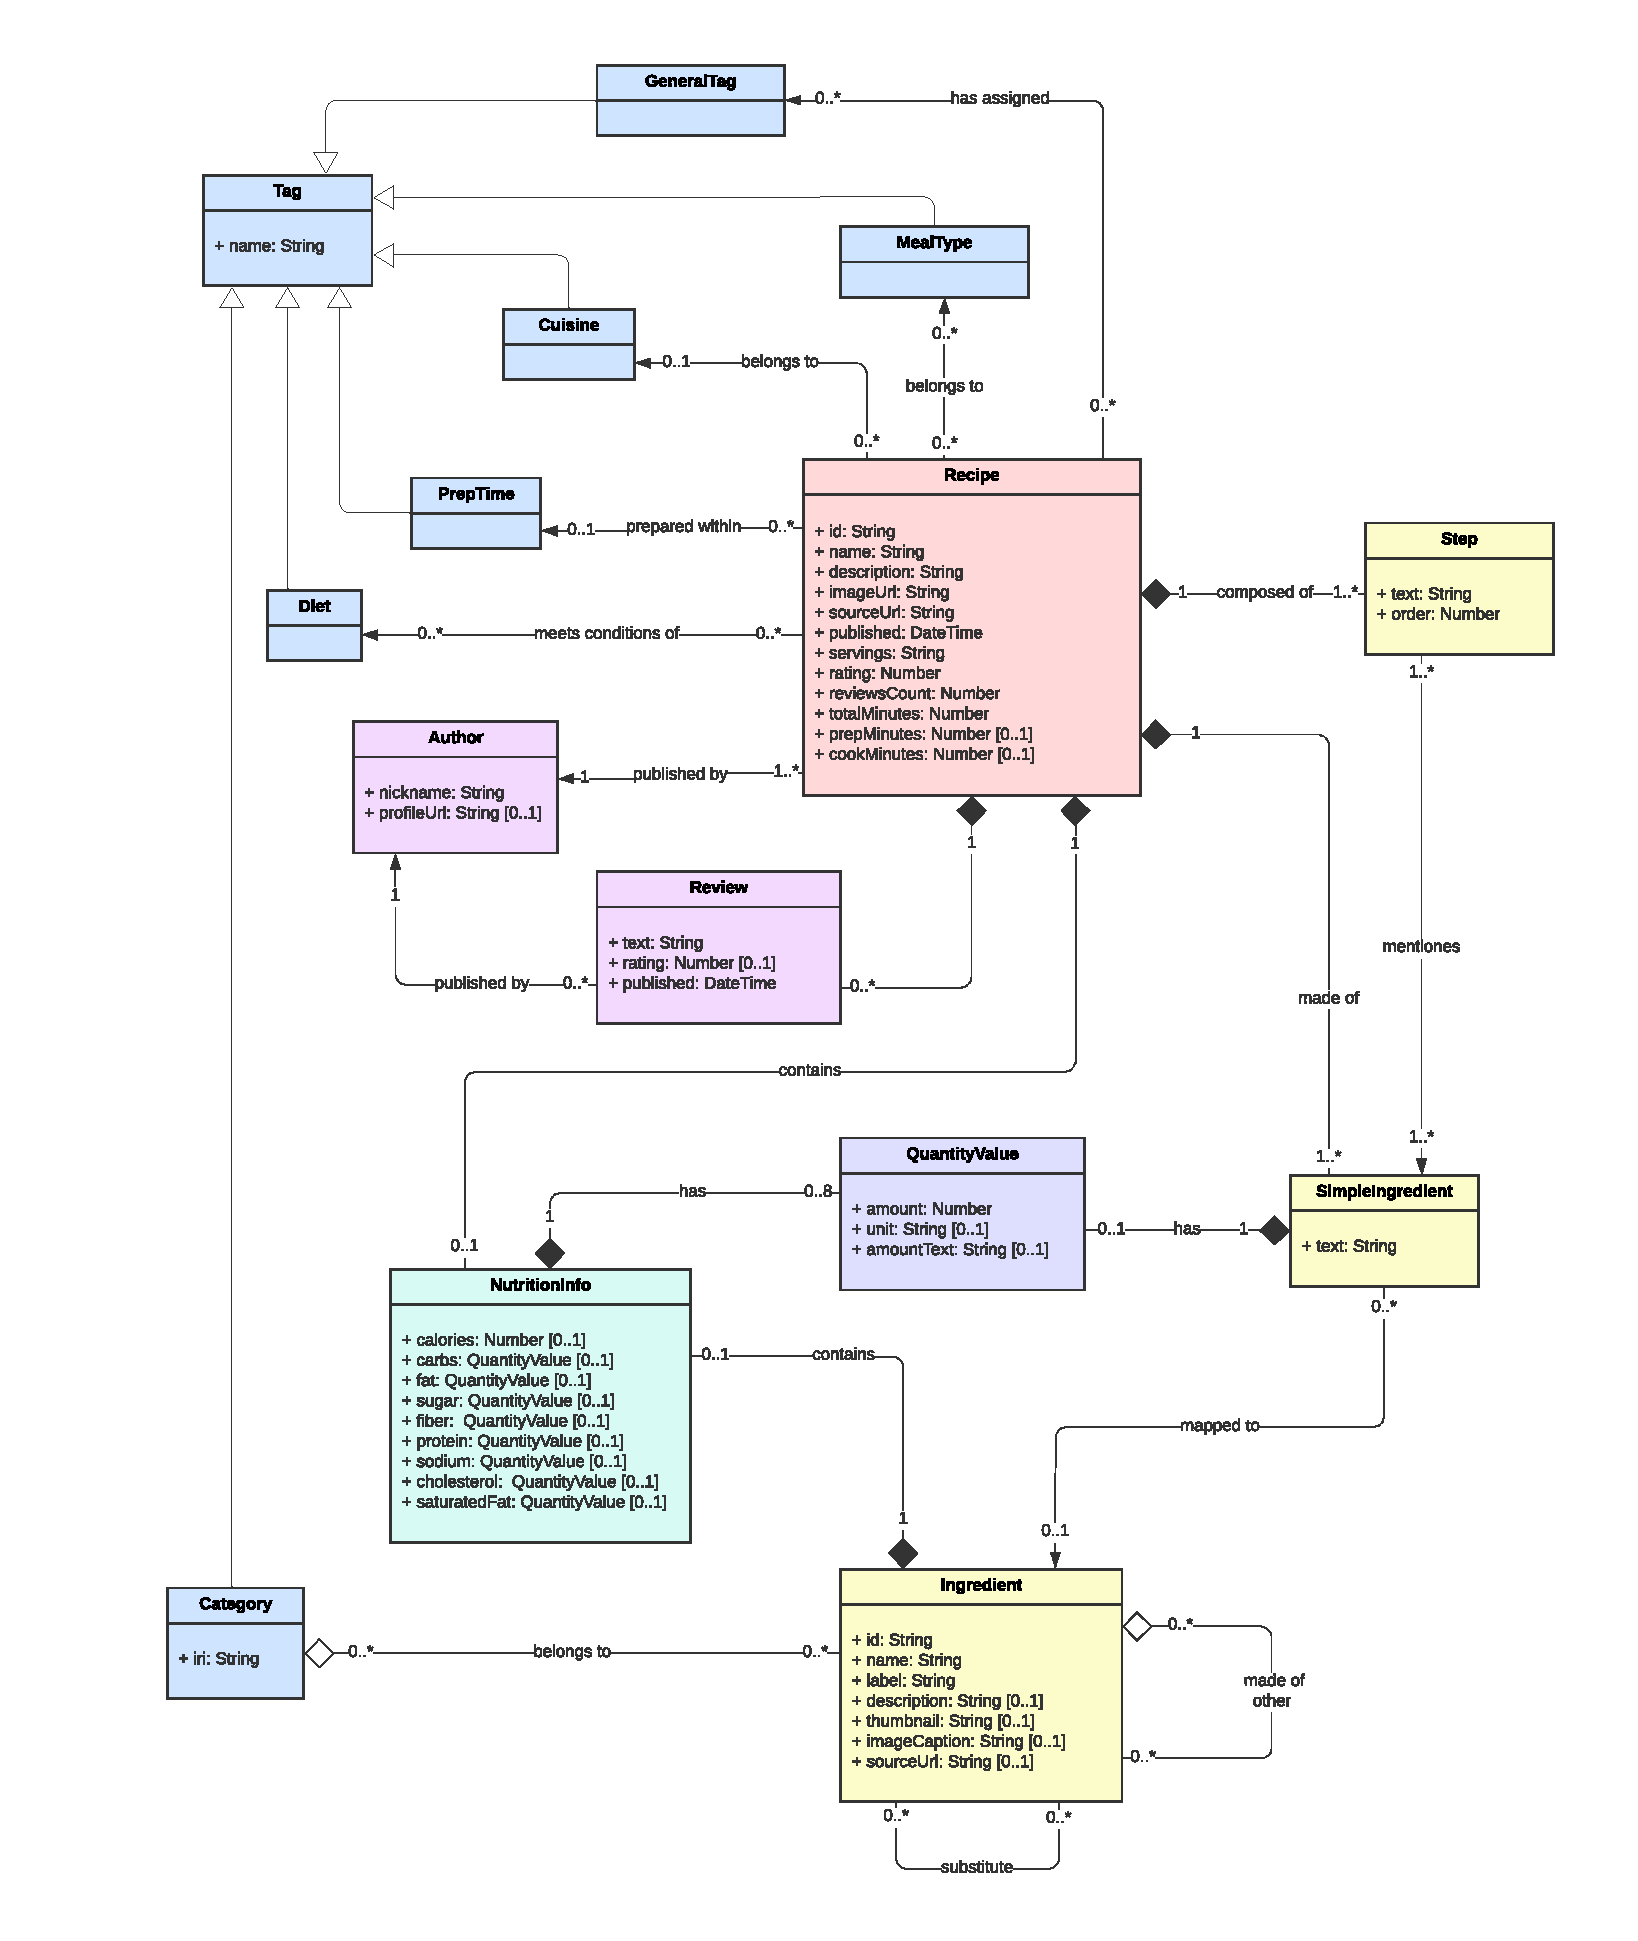
\includegraphics[width=145mm]{../img/conceptual-diagram}
\caption{Konceptuální UML class diagram domény receptů.}
\label{obr01:conceptual-diagram}
\end{figure}